\documentclass[12pt,letterpaper,oneside,titlepage,final]{dalthesis}
\makeindex 


% REMEMBER TO TURN GEOMETRY TO HAVE A MARGIN ON EVERY 2ND PAGE WHEN PRINTING

%Useful Packages
\usepackage[left=1.5in, 
            right=1.0in, 
            top=1.0in, 
            bottom=1.0in]{geometry}%Dal FGS requires 1.5" on left, 1" on all others.
\usepackage{lipsum}                %For \lipsum[2-3]
\usepackage{framed}                %For \begin{framed}
\usepackage{mathtools}             %Extension of amsmath package
\usepackage{graphicx}              %Extension of graphic package.
\usepackage[colorlinks,pdfusetitle]{hyperref}%Makes references clickable links
\usepackage[capitalize]{cleveref}  %Formats equation/table/figure references intelligently.
\usepackage{array}                 %Extending the array and tabular environments
\usepackage{booktabs}              %Publication quality tables in LaTeX
\usepackage{listings}              %Typeset source code listings using LaTeX
\usepackage{float}                 %Improved interface for floating objects
\usepackage[section]{placeins}     %Control float placement
\usepackage{verbatim}              %Reimplementation of and extensions to LaTeX verbatim
\usepackage{enumitem}              %Controls layout of enumerate, itemize and description
\usepackage{caption, subcaption}   %Adds \begin{subfigure} to existing figures.
\usepackage{fancyhdr}              %Adds fancy headers 
\usepackage{bm}                    %Outdated package that still works for bolding greek letters.
\usepackage{indentfirst}           %Indents the first paragraph after new sections
\usepackage{amssymb}               %Adds \mathbb fonts which is used for real numbers R for instance.
\usepackage{mathrsfs}              %Adds \mathscr{} which is just extra script math characters.
\usepackage{physics}               %Adds \abs{} and other physics related commands
\usepackage{braket}                %Adds \braket{0|0}, \bra{0}, or \ket{0}
\usepackage{chemformula}           %To typeset a chemical formula, use \ch{1/2 H2O}
\usepackage{arydshln}              %Can add dashed lines to array via \begin{array}{c;{2pt/2pt}c}
\usepackage{upgreek}               %To get \uppi and \upalpha for instance
\usepackage[toc,page]{appendix}    %For appendices
\usepackage{abstract}              %For better abstract
\usepackage{titlesec}              %Alternative section titles
\usepackage{setspace}              %Control line spacing within a document, \singlespacing, etc
\usepackage{multirow}              %Used for multi-spanning rows in Delocalization error paper
\usepackage{mwe}                   %Used to load example-image
\usepackage{multicol}              %Used for list of symbols and abbreviations 


% LIST OF ABBREVIATIONS SETUP
\setlength{\columnseprule}{0.4pt} % Add vertical line between columns
\newlength{\symwidth}             % Define "symwidth" so the symbol width can vary as needed
\setlength{\symwidth}{1.5cm}      % Set initial length to be 1.5cm
% The \sym command can be used to add a symbol (#1) and a description (#2) to the list of symbols and abbreviations. 
% \makebox[\symwidth][l]{#1}     - Creates a left-aligned left column of width = \symwidth
% \begin{minipage}[t]{width}     - Creates a top-aligned textbox for the description, allowing text to wrap across multiple lines.
% \dimexpr                       - \dimexpr is "dimension expression" allowing you to add dimensions together in a stable way.
% \linewidth-\symwidth\relax     - The width of the minipage becomes \linewidth-\symwidth. \relax ends the calculation safely. 
% \par\vspace{-0.3em}            - Modify this value to change the vertical spacing between entries
\newcommand{\sym}[2]{%
  \noindent\makebox[\symwidth][l]{#1}%
  \begin{minipage}[t]{\linewidth-\symwidth}
  #2
  \end{minipage}\par\vspace{-0.3em}
}
% The \symheader command is used to insert header lines in the List of Abbreviations. It's mostly just custom spacing and adding
% horizontal lines, making use of \sym directly to ensure the spacing via \symwidth stays consistent.
\newcommand{\symheader}[2]{%
  \noindent\rule{\linewidth}{0.6pt}\par
  \vspace{-0.8em}%
  \sym{\textbf{#1}}{\textbf{#2}}\par
  \vspace{-1.0em}%
  \noindent\rule{\linewidth}{0.6pt}\par
  \vspace{0.4em}%
}

% BIBLIOGRAPHY SETUP
\usepackage[utf8]{inputenc} %Needed for some citations
\DeclareUnicodeCharacter{1EF3}{\`y}
\DeclareUnicodeCharacter{1E81}{\`w}
\usepackage[backend=biber,
            backref=true,
            backrefstyle=two,
            maxbibnames=10,
            minbibnames=10,
            sorting=none, 
            giveninits=true,
            doi=true,
            intitle=true,
            articletitle=true,
            style=nature]{biblatex}
    \DefineBibliographyStrings{english}{
        backrefpage={p.},
        backrefpages={p.}
    }
    \addbibresource{Bibliography.bib}    

% CLEVERREF SETUP
  \Crefname{equation}{Eq.}{Eqs.}
  \Crefname{chapter}{Chapter}{Chapters}
  \Crefname{section}{Section}{Sections}
  \Crefname{figure}{Figure}{Figures}
  \Crefname{tabular}{Table}{Tables}
  \Crefname{table}{Table}{Tables}
  \hypersetup{
    colorlinks=true,
    citecolor=blue,
    linkcolor=blue,
    filecolor=magenta,      
    urlcolor=cyan,
  }


% CUSTOM COMMANDS
  \newcommand{\e}{\mathrm{e}}    %Exponential
  \renewcommand{\i}{\mathrm{i}}  %Imaginary Number 
  \renewcommand{\pi}{\uppi}      %Convert all pi to upright. I'll never need italicized.
  \newcommand*{\doi}[1]{doi: #1} %Used to easily add DOIs if needed

% FANCYHEADER SETUP
  %\renewcommand{\chaptermark}[1]{\markboth{\footnotesize \MakeUppercase{#1}}{}}
  %\renewcommand{\sectionmark}[1]{\markright{\footnotesize \MakeUppercase{#1}}}
  \setlength{\headheight}{15pt} %Fancyhdr gives warnings unless this value is at least 14.49998pt. 
  \fancypagestyle{Body}{%This will work for section headers
	\fancyhf{}
	\fancyhead[R]{\thepage}
	\fancyhead[L]{\S\rightmark}
  }
  \fancypagestyle{Chapter}{%This will work for chapter headers
	\fancyhf{}
	\fancyhead[R]{\thepage}
	\fancyhead[L]{\leftmark}
  }
  \renewcommand{\bibsetup}{\thispagestyle{Chapter}\pagestyle{Chapter}}

% DAL FGS SETUP
  \allowdisplaybreaks
  \numberwithin{equation}{section}
  \raggedbottom
  \captionsetup{width=0.9\textwidth}
  \setlength{\tabcolsep}{2.5pt}
  \setitemize{itemsep=-0.5em} 
  \hbadness=4000              % Stops the "Underfull \hbox" warnings
  \setlength{\parskip}{0.5em} % Adds slight spacing between paragraphs without need for //
  \onehalfspacing             % Dal FGS Requires \onehalfspacing or \doublespacing
                              % Switch to \singlespacing for TOC/LOF/LOT/Bib, then switch back.


% TITLE PAGE SETUP
  \renewcommand{\contentsname}{Table of Contents}
  \newcommand{\ThesisAuthor}{Author's-Name}
  \newcommand{\ThesisTitle}{Title-of-Thesis}
  \newcommand{\ThesisDegree}{Title-of-Degree}%Doctor of Philosophy / Master of Science
  \newcommand{\ThesisMonth}{Month-of-Defence}
  \newcommand{\ThesisYear}{Year-of-Defence}
  \newcommand{\ThesisAdvisor}{Professor-Name}
  \newcommand{\ThesisUniversity}{Dalhousie University}
  \newcommand{\ThesisLocation}{Halifax, Nova Scotia}
  \newcommand{\ThesisLandAcknowledgement}{Dalhousie University is located in the Mi'kma'ki, the\\%
	                                     ancestral and unceded territory of the Mi'kmaq.\\%
	                                     We are all Treaty people.%
	                                     }
  \newcommand{\skiplines}[1]{\vspace{#1\baselineskip}}


\begin{document} 
\pagenumbering{roman}

\begin{titlepage}
\centering
\vspace*{\fill}
\textsc{\textbf{\large{\ThesisTitle}}}\\%
\skiplines{2}%
\textbf{
	{\!}by\\% Small negative space corrects block kerning issues for small lines caused by textbf
	\skiplines{2}%
	\ThesisAuthor\\%
	\skiplines{6}%
	Submitted in partial fulfilment of the requirements\\%
	for the degree of \ThesisDegree\\%\ in \ThesisProgram\\
	\skiplines{2}%
	{\!}at\\% Small negative space corrects block kerning issues for small lines caused by textbf
	\skiplines{2}%
	\ThesisUniversity\\%
	\ThesisLocation\\%
	\ThesisMonth, \ThesisYear\\%
	\skiplines{2}%
	\ThesisLandAcknowledgement\\%
	\skiplines{4}%
	\copyright\ Copyright by \ThesisAuthor, \ThesisYear%
}
\vspace{\fill} % centers title page vertically
\end{titlepage}


%~~~~~~~~~~~~~~~~~~~~~~~~~~~~~~~~~~~~~~~~~~~~~~~~~~~~~~~~~~~~~~~~~~~~~~~~~~~~~~~~~~~~~~~~~~~~~~~~
\chapter*{\centering\large\textsc{Dedication}} \setcounter{page}{2}
%~~~~~~~~~~~~~~~~~~~~~~~~~~~~~~~~~~~~~~~~~~~~~~~~~~~~~~~~~~~~~~~~~~~~~~~~~~~~~~~~~~~~~~~~~~~~~~~~
\vspace*{6cm}
\begin{center}
\large 
\noindent{}Dedication Goes Here (Optional)\\
\noindent{}$\mathbf{\dots}$\\
\end{center}
\clearpage





%~~~~~~~~~~~~~~~~~~~~~~~~~~~~~~~~~~~~~~~~~~~~~~~~~~~~~~~~~~~~~~~~~~~~~~~~~~~~~~~~~~~~~~~~~~~~~~~~
\chapter*{\centering\large\textsc{Preface}} 
%~~~~~~~~~~~~~~~~~~~~~~~~~~~~~~~~~~~~~~~~~~~~~~~~~~~~~~~~~~~~~~~~~~~~~~~~~~~~~~~~~~~~~~~~~~~~~~~~

I want to start by acknowledging that this Dalhousie thesis template is built on a slightly modified version of the \texttt{ocethesis.cls} class, maintained by Prof.\@ Dan Kelley on his personal GitHub \href{https://github.com/dankelley/dal-oce-thesis}{( github.com/dankelley/dal-oce-thesis )}. This work branched off somewhere around 2015, and the \texttt{ocethesis} class was eventually passed from student to student until it reached me. Over the years, I've tweaked it to suit my own style while fixing some issues that arose due to deprecated packages, and whatever else happens to old code when you haven't looked at it for a few months. I thank the previous contributors to this \TeX\ class file, Dan Kelley, Vlado Keselj, Mike McAllister, Clyde Clements, Steven Matheson, Joseph Pallas, and others whom I have missed. 

This class file, now renamed to \texttt{dalthesis.cls}, is hosted alongside this thesis \texttt{.tex} template on my GitHub \href{https://github.com/KyleBryenton/Dalhousie-LaTeX-Templates}{( github.com/KyleBryenton/Dalhousie-LaTeX-Templates )} to help take some of the pain out of the thesis writing process for future Dalhousie graduate students. This template is geared towards disciplines like chemistry or physics, and it adheres to Dalhousie Faculty of Graduate Studies (FGS) format requirements as of Summer 2025. An example of a completed thesis using this template can be seen here: \href{https://dalspace.library.dal.ca/items/2f33c6cd-166c-4031-bc01-ba1deaab62b7}{( dalspace.library.dal.ca/items/2f33c6cd-166c-4031-bc01-ba1deaab62b7 )}. I've left various packages and settings in the template that I found helpful during my writing process, complete with comments to help clarify what these packages can be used for.

This template uses a compact ``List of Abbreviations and Symbols'' that some theory-heavy students may find desirable. This compact template avoids having potentially one or two dozen pages dedicated to that part of the front matter. I've tried to make this as user-friendly as possible. The comments in that section of the \texttt{.tex} will guide you, and my full lists remain intact to serve as examples.\\

The bibliography is set up to use a provided \texttt{.bib} file using Biber (not Bib(La)TeX) as the backend. Some installations will automatically adjust to use Biber (such as Overleaf), but others may require you to change your compilation settings. I've left some citations in this template to showcase the bibliography format. The reference style expands on the ``Nature'' format by including additional information such as full article names, full author lists, digital online identifiers (DOIs), and back references (adds hyperlinks to a reference pointing to each page it was cited in the manuscript). To help compile your bibliography file, I recommend the Google Scholar Button extension (on Chromium-based browsers, Firefox, and others) to generate the \texttt{bibtex} entries. You will sometimes need to add the pages and DOI fields manually, check author lists to convert unicode accents to \TeX, ensure the entry doesn't cap the number of authors listed and end with ``and others'', and manually abbreviate the name of the journal used. To consistently abbreviate journal names, I highly recommend UBC's Woodward Library Science and Engineering Journal Abbreviations tool: \href{https://woodward.library.ubc.ca/woodward/research-help/journal-abbreviations/}{( woodward.library.ubc.ca/woodward/research-help/journal-abbreviations/ )}.

The final step for submitting your thesis is to convert to PDF/A-1b format. However, this process can be quite tricky. To convert to PDF/A-1b, I used \href{https://xodo.com/pdf-to-pdfa}{( xodo.com/pdf-to-pdfa )} and to validate I used \href{https://www.pdfforge.org/online/en/validate-pdfa}{( www.pdfforge.org/online/en/validate-pdfa )}. If your \texttt{tikz} graphics are affected by this conversion, it may be due to lack of support for RGBA values. Convert your RGBA values to plain RGB, and ensure all fill opacity values used in your \texttt{tikz} are set to \texttt{fill opacity=1.0}. If this conversion causes compression of any graphics used in your thesis, I was able to alleviate this by converting PNG $\rightarrow$ PDF (at 1$\times$ scale) $\rightarrow$ PDF (at 3$\times$ scale) using GIMP for the affected images.

Lastly, I made this template based on my own personal preferences, and any advice or suggestions offered here reflect that. If your advisor, committee, department, or faculty disagree with anything in this template, please defer to their input over my own. I hope you find this template useful.


\clearpage




\singlespacing              % Use more compact spacing in TOCs / Lists
\interlinepenalty=10000	    % Forces no pagebreaks
%~~~~~~~~~~~~~~~~~~~~~~~~~~~~~~~~~~~~~~~~~~~~~~~~~~~~~~~~~~~~~~~~~~~~~~~~~~~~~~~~~~~~~~~~~~~~~~~~
\tableofcontents                                                 \clearpage
\listoftables    \addcontentsline{toc}{chapter}{List of Tables}  \clearpage
\listoffigures   \addcontentsline{toc}{chapter}{List of Figures} \clearpage
%~~~~~~~~~~~~~~~~~~~~~~~~~~~~~~~~~~~~~~~~~~~~~~~~~~~~~~~~~~~~~~~~~~~~~~~~~~~~~~~~~~~~~~~~~~~~~~~~
\onehalfspacing             % Switch back to default
\interlinepenalty=0    	    % Switch back to default







%~~~~~~~~~~~~~~~~~~~~~~~~~~~~~~~~~~~~~~~~~~~~~~~~~~~~~~~~~~~~~~~~~~~~~~~~~~~~~~~~~~~~~~~~~~~~~~~~
\chapter*{\centering\large\textsc{Abstract}}  \addcontentsline{toc}{chapter}{Abstract} 
%~~~~~~~~~~~~~~~~~~~~~~~~~~~~~~~~~~~~~~~~~~~~~~~~~~~~~~~~~~~~~~~~~~~~~~~~~~~~~~~~~~~~~~~~~~~~~~~~

As of 2025, Dalhousie's Faculty of Graduate Studies (FGS) Thesis Format Guidelines require the abstract to be one page. It may be single-spaced if necessary, but it must not include illustrations or footnotes. Note that abstracts archived by the library are truncated to 150 words for MSc theses and 350 words for PhD theses. A good abstract should summarize the work and frame it within a common theme, rather than discussing a series of disjointed papers. This is where you introduce the reader to that flow.




%~~~~~~~~~~~~~~~~~~~~~~~~~~~~~~~~~~~~~~~~~~~~~~~~~~~~~~~~~~~~~~~~~~~~~~~~~~~~~~~~~~~~~~~~~~~~~~~~
\chapter*{List of Abbreviations and Symbols Used}
\addcontentsline{toc}{chapter}{List of Abbreviations and Symbols Used}
%~~~~~~~~~~~~~~~~~~~~~~~~~~~~~~~~~~~~~~~~~~~~~~~~~~~~~~~~~~~~~~~~~~~~~~~~~~~~~~~~~~~~~~~~~~~~~~~~

% INSTRUCTIONS FOR HOW TO GENERATE LIST OF ABBREVIATIONS AND SYMBOLS
%
% 1. Entries should be added using the custom \sym command. (e.g.):
%        \sym{ $\pi$ }{ Pi, the ratio of a circle's circumference to its diameter ($=3.14159265\ldots$)} 
%
% 2. I suggest manually placing columnbreaks are and add a new header using the \symheader command. (e.g.):
%        \columnbreak
%        \symheader{Symbol}{Description}
%
% 3. To add a new category within a table, I suggest adding a space before, and a \par after. (e.g.):
%        \vspace*{1em}
%        \textit{\textbf{Common or fundamental constants}}\par
%
% 4. Use \setlength{\symwidth}{1.3cm} to decide the spacing between the first and second parts of your
%    headings. I found around 1.3cm was good for math symbols, and 1.7cm was good for abbreviations.
%
% If your multicols enviroment ends with enough space to not fully fill the first column, it will try
% to balance what remains between both columns. If you would rather it fill the left column completely
% use \begin{multicols*}{2} rather than \begin{multicols}{2}. Between multicols (i.e. one used for 
% symbols, and another used for abbreviations) I suggest using a \clearpage or a \vspace*{1cm} between
% them to visually separate them. For font size, I suggest using \scriptsize or \footnotesize. Both 
% are acceptable and will pass Dalhousie FGS guidelines. 

\scriptsize
\begin{multicols}{2} \setlength{\symwidth}{1.3cm}
\symheader{Symbol}{Description}
\vspace*{1em}
\textit{\textbf{General symbols and notation}}\par

\sym{ $\text{a}$ }{ Constant (upright, non-bold) } 
\sym{ $a$ }{ Variable (italic, non-bold) } 
\sym{ $\bm{a}$ }{ Vector (italic, bold)}
\sym{ $\textbf{a}$ }{ Tensor (upright, bold) }
\sym{ $\hat{a}$ }{ Operator (italic, non-bold, hat) }
\sym{ $\hat{\text{a}}$ }{ Unit vector (upright, non-bold, hat) }
\sym{ $a'$ }{ Derivative of $a$ }
\sym{ $\frac{d}{dr}a$ }{ Derivative of $a$ with respect to $r$ }
\sym{ $\frac{\delta}{\delta r}a$ }{ Functional derivative of $a$ with respect to $r$}
\sym{ $\Delta a$ }{ Change in $a$ }
\sym{ $\nabla a$ }{ Gradient of $a$ }
\sym{ $\nabla \cdot \bm{a}$ }{ Divergence of $\bm{a}$ }
\sym{ $\nabla \cross \bm{a}$ }{ Curl of $\bm{a}$ }
\sym{ $\nabla^{2} a$ }{ Laplacian of $a$ }
\sym{ $\nabla \otimes \textbf{a}$ }{ Tensor product of $\nabla$ and $\textbf{a}$ }
\sym{ $\textbf{a}^{-1}$ }{ Matrix inverse of $\textbf{a}$ }
\sym{ $\textbf{a}^{\textsf{T}}$ }{ Matrix transpose of $\textbf{a}$ }
\sym{ $\tr[\textbf{a}]$ }{ Trace of matrix $\textbf{a}$ }
\sym{ $\Bra{a_{i}}$ }{ Row vector of $a_{i}$ }
\sym{ $\Ket{a_{i}}$ }{ Column vector of $a_{i}$ }
\sym{ $\Braket{a}$ }{ Expectation value of $a$ (see Dirac notation)}

\vspace*{1em}
\textit{\textbf{Common or fundamental constants}}\par

\sym{ \textbf{1} }{ Ones matrix, a matrix where every element is 1 }
\sym{ \AA }{ Angstrom, ($=10^{-10} \text{ m}$) }
\sym{ $a_{0}$ }{ Bohr radius, the mean radius between an electron and the nucleus for the ground-state H atom ($=1\text{ a.u.}$)}
\sym{ $\e$ }{ Euler's number, the base of the natural logarithm ($=2.71828182\ldots$)}
\sym{ $e$ }{ Charge of an electron ($=1\text{ a.u.}$)}

\columnbreak
\symheader{Symbol}{Description}

\sym{ $h$ }{ Planck's constant, equal to a photon's energy divided by its frequency}
\sym{ $\hbar$ }{ Reduced Planck's constant, ($=\nicefrac{h}{2\pi}=1\text{ a.u.}$) }
\sym{ $\textbf{I}$ }{ Identity matrix, a square matrix with ones on the main diagonal and zeros elsewhere }
\sym{ $\i$ }{ Imaginary number, solution to $x^2=-1$ } 
\sym{ $\epsilon_{0}$ }{ Permittivity of free space ($4\pi\epsilon_{0} = 1 \text{ a.u.}$) }
\sym{ $\pi$ }{ Pi, the ratio of a circle's circumference to its diameter ($=3.14159265\ldots$)} 

\vspace*{1em}
\textit{\textbf{Used atomic orbitals}}\par

\sym{ $s$ }{ $1s$, $2s$ }
\sym{ $p$ }{ $2p_{x}$, $2p_{y}$, $2p_{z}$, $3p_{x}$, $3p_{y}$, $3p_{z}$  }
\sym{ $d$ }{ $3d_{z^{2}}$, $3d_{xz}$, $3d_{yz}$, $3d_{xy}$ , $3d_{x^{2}-y^{2}}$ }
\sym{ $f$ }{ $4f_{z^{3}}$, $4f_{xz^{2}}$, $4f_{yz^{2}}$, $4f_{xyz}$, $4f_{z(x^{2}-y^{2})}$, $4f_{x(x^{2}-3y^{2})}$, $4f_{y(3x^{2}-y^{2})}$  }

\vspace*{1em}
\textit{\textbf{Used indices \& their typical groupings}}\par

\sym{ \hspace*{2em} $\cdot$ }{ $A$, $B$, $C$}
\sym{ \hspace*{2em} $\cdot$ }{ $a$, $b$, $c$}
\sym{ \hspace*{2em} $\cdot$ }{ $i_{1}$, $i_{2}$, $i_{3}$, $i_{4}$}
\sym{ \hspace*{2em} $\cdot$ }{ $i$, $j$, $k$ }
\sym{ \hspace*{2em} $\cdot$ }{ $k$, $\ell$, $m$ }
\sym{ \hspace*{2em} $\cdot$ }{ $m$, $n$ }
\sym{ \hspace*{2em} $\cdot$ }{ $p$, $q$ }
\sym{ \hspace*{2em} $\cdot$ }{ $\alpha$, $\beta$, $\gamma$ }
\sym{ \hspace*{2em} $\cdot$ }{ $\sigma$, $\sigma^{\prime}$ }
\sym{ \hspace*{2em} $\cdot$ }{ $\mu$, $\nu$ }

\vspace*{1em}
\noindent\rule{\linewidth}{0.6pt}

\vspace*{1em}
\noindent For a complete example with a list for abbreviations and another for Latin and Greek mathematical symbols, un-comment the 2nd and 3rd tables in \texttt{thesis\_template.tex}\par

\vspace*{1em}
\noindent\rule{\linewidth}{0.6pt}

\end{multicols}
\normalsize

%% For a complete list with a list of abbreviations, and Latin and Greek mathematical symbols, 
%% un-comment the 2nd and 3rd tables below
%\scriptsize
%\clearpage
%\begin{multicols}{2} \setlength{\symwidth}{1.7cm}
%\symheader{Abbrev.\@}{Description}
\vspace*{1em}
\textit{\textbf{General Abbreviations}}\par

\sym{ A$_m$H$_n$ }{ Hydride with stoichiometric coefficients $m$ and $n$ }
\sym{ ACFD(T) }{ Adiabatic connection fluctuation-dissipation theorem }
\sym{ ADF }{  Amsterdam Density Functional }
\sym{ AMS }{  Amsterdam Modelling Suite }
\sym{ AE }{ All-electron }
\sym{ APW }{ Augmented planewave method }
\sym{ ATM }{ Axilrod--Teller--Muto triple-dipole dispersion energy term } 
\sym{ Abs }{ Absolute (e.g., Ice13(Abs) absolute energy }
\sym{ a$N$Z }{ Augmented $N$-zeta Dunning basis set }
\sym{ a.u.\ }{ (Hartree) atomic unit } 

\sym{ B3LYP }{ Becke, 3-parameter, Lee--Yang--Parr hybrid density functional }
\sym{ B86a }{ Becke's B86a GGA density functional }
\sym{ B86b }{ Becke's B86b GGA density functional }
\sym{ B86bPBE }{ Becke's B86b exchange with PBE correlation GGA density functional } 
\sym{ B86bPBE0 }{ Becke's B86b exchange with PBE correlation hybrid density functional } 
\sym{ B88 }{  Becke's B88 GGA density functional }
\sym{ BHLYP }{ Becke and Lee--Yang--Parr ``half and half'' hybrid density functional }
\sym{ BJ }{ Becke--Johnson damping function (e.g. XDM(BJ)) }
\sym{ BO }{ Born--Oppenheimer approximation }
\sym{ BR }{ Becke--Roussel exchange hole } 
\sym{ BSC }{ Basis set corrected }

\sym{ C }{ Correlation }
\sym{ CBS }{ Complete basis set }
\sym{ CC }{ Coupled-cluster theory (e.g. CCSD) }
\sym{ CCSD(T) }{ CC theory with singles, doubles and perturbative triple excitations }
\sym{ CFDM }{ Coupled fluctuating dipole model }
\sym{ CI }{ Configuration interaction method }
\sym{ CHG }{ Chai and Head--Gordon damping function }
\sym{ CN }{ Coordination number }
\sym{ CP }{ Counterpoise } 
\sym{ CPU }{ Central processing unit } 
\sym{ CSP }{ Crystal structure prediction }
\sym{ ca. }{ circa (=about) }

\columnbreak
\symheader{Abbrev.\@}{Description}

\sym{ cc-p }{ Correlation-consistent and polarized (e.g. aug-cc-pVTZ) }
\sym{ D/DC }{ Dispersion corrected (e.g. DFT-D or DC-DFT) }
\sym{ DC }{ Dynamical correlation }
\sym{ DFA }{ Density-functional approximation }
\sym{ DFT }{ Density-functional theory }
\sym{ D$n$ }{ Grimme's series of dispersion corrections (e.g., DFT-D$n$, $n$= 1, 2, 3, 4) }
\sym{ DMC }{ Diffusion Monte Carlo method }
\sym{ DOS }{ Dipole oscillator strength }
\sym{ DOSD }{ Dipole oscillator strength distribution }
\sym{ dDsC }{ Steinmann and Corminboeuf's density- dependent dispersion correction }
\sym{ d }{ Damping }

\sym{ Eq. }{ $\cdot$ Equilateral triangle }
\sym{     }{ $\cdot$ Equation }
\sym{ Eqs. }{ Equations }
\sym{ E$_\text{h}$ }{ One hartree of energy }
\sym{ eV }{ Electron volt }

\sym{ F12 }{ Explicit correlation method (a.k.a. R12) }
\sym{ FCI }{ Full configuration interaction }
\sym{ FFT }{ Fast (discrete) Fourier transform }
\sym{ FHI-aims }{ Fritz Haber Institute \textit{ab initio} materials simulations }
\sym{ FI }{ Fractionally ionic (e.g., MBD/FI) }
\sym{ FN }{ Fixed-node approximation }

\sym{ GGA }{ Generalized-gradient approximation } 
\sym{ GMTKN55 }{ General main-group thermochemistry, kinetics, and non-covalent interactions }
\sym{ GTO }{ Gaussian-type orbitals }

\sym{ HF }{ Hartree--Fock theory } 
\sym{ HF-D }{ Scoles' dispersion-corrected Hartree--Fock  method }
\sym{ HI }{ Iterative Hirshfeld partitioning scheme (e.g. MBD/HI) }
\sym{ HSE06 }{ Heyd--Scuseria--Ernzerhof variable exchange hybrid functional }
\sym{ Ha. }{ Hartree (unit) }
\sym{ HalCrys4 }{ Halogen crystal benchmark }

\sym{ Ice13 }{ The Ice13 ice polymorph lattice energy benchmark }
\sym{ IBZ }{ Irreducible Brillouin zone }
\sym{ Iso. }{ Isomerizations }

\sym{ KB49 }{ Kannemann--Becke benchmark set of 49 molecular dimers } 

\columnbreak
\symheader{Abbrev.\@}{Description}

\sym{ KB65 }{ Kannemann--Becke benchmark set of 65 molecular dimers } 
\sym{ kcal }{ Kilocalorie }
\sym{ KS }{ Kohn--Sham (e.g., KS-DFT) }

\sym{ LAPW }{ Linearized augmented planewave methods }
\sym{ LDA }{ Local-density approximation } 
\sym{ LJ }{ Lennard-Jones potential }
\sym{ LSDA }{ Local spin-density approximation } 
\sym{ Lin. }{ Linear }

\sym{ M }{ Mooij (e.g., $f^{\text{M}}$ damping) }
\sym{ MAD }{ Mean absolute deviation }
\sym{ MAE }{ Mean absolute error }
\sym{ MAPD }{ Mean absolute percent deviation }
\sym{ MAPE }{ Mean absolute percent error }
\sym{ MAX }{ Maximum absolute error }
\sym{ MBD }{ Many-body dispersion model } 
\sym{ MBDQ }{ Many-body dispersion model with quadrupole interactions } 
\sym{ MD }{ Mean deviation }
\sym{ ME }{ Mean error }
\sym{ mGGA }{ Meta-generalized gradient approximation }
\sym{ MolC6 }{ Molecular $C_6$ dispersion coefficient benchmark by Johnson and Becke }
\sym{ MP }{ Monkhorst--Pack $\bm{k}$-point grid sampling scheme } 
\sym{ MP2 }{ M\o{}ller--Plesset second-order perturbation theory } 
\sym{ MP2C }{ MP2 coupled method }

\sym{ NAO }{ Numerical atom-centred orbitals }
\sym{ NC }{ Norm-conserving (e.g., pseudopotential) }
\sym{ NCI }{ Non-covalent interactions }
\sym{ NDC }{ Non-dynamical correlation }
\sym{ NI }{ Non-interacting }
\sym{ NL }{ Non-local (e.g. MBD-NL) }
\sym{ NLDF }{ Non-local density functional 
}
\sym{ Opt. }{ Optimization }

\sym{ PAW }{ Projector-augmented wave } 
\sym{ PBE }{ Perdew--Burke--Ernzerhof GGA density functional } 
\sym{ PBE0 }{ Perdew--Burke--Ernzerhof hybrid density functional }
\sym{ PES }{ Potential energy surface } 
\sym{ PP }{ Pseudopotential }
\sym{ PRO }{ Percent radial overlap }

\columnbreak
\symheader{Abbrev.\@}{Description}

\sym{ PT(2) }{ Perturbation theory, (second-order) }
\sym{ PVO }{ Percent volume overlap }
\sym{ PW86 }{ Perdew-Wang PW86 GGA density functional } 
\sym{ p. }{ Page }

\sym{ QE }{ Quantum ESPRESSO } 
\sym{ QHO }{ Quantum harmonic oscillator }
\sym{ QMC }{ Quantum Monte Carlo }

\sym{ RFA }{ Response-function approximation }
\sym{ RMSD }{ Root mean squared deviation }
\sym{ RMSPD }{ Root mean squared percent deviation }
\sym{ RMSE }{ Root mean squared error }
\sym{ RMSPE }{ Root mean squared percent error }
\sym{ RPA }{ Random-phase approximation }
\sym{ RPA-3 }{ RPA's three-body-only energy }
\sym{ RS }{ Range separation }
\sym{ Rel }{ Relative (e.g. Ice13(Rel) relative energies) }
\sym{ Ri. }{ Right-angle triangle }
\sym{ Ry }{ Rydberg }
\sym{ rsSCS }{ Range-separated self-consistent screening }
\sym{ rVV10 }{ Revised Vydrov and van Voorhis non-local density functional } 

\sym{ S12L }{ Grimme's large complexes benchmark  }
\sym{ S22 }{ Benchmark set of non-covalent complexes }
\sym{ S66 }{ Benchmark set of 66 gas-phase dimers }
\sym{ S66$\times$7 }{  Benchmark set of 66 gas-phase dimers  with 7 inter-fragment distances }
\sym{ S66$\times$8 }{  Benchmark set of 66 gas-phase dimers  with 8 inter-fragment distances }
\sym{ SCF }{ Self-consistent field } 
\sym{ SCS }{ Self-consistent screening } 
\sym{ SIE }{ Self-interaction error }
\sym{ STO }{ Slater-type orbital }

\sym{ TMDC }{ Transition-metal dichalcogenides }
\sym{ TPSS }{ Tao--Perdew--Staroverov--Scuseria mGGA functional }
\sym{ TS }{ Tkatchenko--Scheffler dispersion model } 
\sym{ TSsurf }{ Tkatchenko--Scheffler dispersion model for surfaces }

\sym{ UEG }{ Uniform electron gas }
\sym{ US }{ Ultra-soft (e.g., pseudopotential) }
\sym{ uMBD }{ Universal many-body dispersion model }

\sym{ V }{ Valence (e.g., pVTZ) }

\columnbreak
\symheader{Abbrev.\@}{Description}

\sym{ VSXC }{ Voorhis and Scuseria's $\tau$-dependent mGGA functional }
\sym{ VV }{ Vydrov and van Voorhis }
\sym{ VV10 }{ Vydrov and van Voorhis non-local density functional }
\sym{ vdW }{ van der Waals } 
\sym{ vdW-DF }{ Dion's van der Waals density functional }
\sym{ vdW-DF2 }{ Lundqvist \& Langreth's van der Waals density functional }

\sym{ W$n$ }{ Weizmann-n methods $n = 1, 2, 3,...$ }
\sym{ WTMAD }{ Weighted mean absolute deviation  (e.g., WTMAD-$n$, $n = 1, 2, 3, 4$) }

\columnbreak
\symheader{Abbrev.\@}{Description}

\sym{ WY }{ Wu--Yang Fermi-type damping function }

\sym{ X }{ Exchange }
\sym{ X23 }{ Benchmark set of molecular organic solids } 
\sym{ XC }{ Exchange correlation }
\sym{ XCDM }{ Exchange-correlation dipole moment dispersion model } 
\sym{ XDM }{ Exchange-hole dipole moment dispersion model } 

\sym{ Z }{ Z-damping function (e.g. XDM(Z)) }
\sym{ ZORA }{ Zero-order regular approximation }

\vspace*{1em}
\noindent\rule{\linewidth}{0.6pt}

%\end{multicols}
%\clearpage
%\begin{multicols}{2} \setlength{\symwidth}{1.5cm}
%\symheader{Symbol}{Description}
\vspace*{1em}
\textit{\textbf{Mathematical Symbols (Latin)}}\par

\sym{ $A$ }{ Normalization constant for BR hole }
\sym{ $\bm{\mathsf{A}}$ }{ MBD@rsSCS RFA polarizability tensor }
\sym{ $\textbf{A}$ }{ SCS interaction tensor }
\sym{ $A,\,B,\,C$ }{ Nuclear index values }
\sym{ $a$ }{ SCAN $\tau$-dependent term }
\sym{ $\overline{a}$ }{ r$^2$SCAN $\tau$-dependent term }
\sym{ $a_{\sigma}$ }{ Exponent of BR-hole orbital for spin $\sigma$ }
\sym{ $a_{\text{latt}}$ }{ Lattice constant }
\sym{ $a_{\text{latt}}^{\text{min}}$ }{ Minimum-energy lattice constant }
\sym{ $a_{\text{latt}}^{\text{rel}}$ }{ Relaxed lattice constant }
\sym{ $a_{1},\,a_{2}$ }{ Becke--Johnson damping parameters }
\sym{ $a,\,b,\,c$ }{ $\cdot$ PW86 parameters }
\sym{            }{ $\cdot$ Lattice constants }
\sym{ $a_{\text{X}}$ }{ Hybrid exchange mixing parameter }
\sym{ $a_{\text{C}}$ }{ Double hybrid correlation mixing parameter }
\sym{ $\bm{a}_{i}$ }{ Primitive/Bravais/real-space lattice vectors }

\sym{ $b_{\sigma}$ }{ BR exchange hole displacement for spin $\sigma$ }
\sym{ $\bm{b}_{i}$ }{ Reciprocal lattice vectors }
\sym{ $b_n,\,\mu$ }{ SCAN $x$-function parameters }

\sym{ $C$ }{ Vydrov and van Voorhis polarizability functional tunable parameter } 
\sym{ $C,\,d,\,\mu$ }{ r$^2$SCAN $x$-function parameters }
\sym{ $C_{6}$ }{ Dipole-dipole dispersion coefficient }
\sym{ $C_{8}$ }{ Dipole-quadrupole dispersion coefficient }
\sym{ $C_{9}$ }{ ATM 3-body nonadditive dispersion  coefficient }
\sym{ $C_{10}$ }{ Dipole-octupole or quadrupole-quadrupole  dispersion coefficient }
\sym{ $C_{12}$ }{ Dipole-hexadecapole or quadrupole-octupole  dispersion coefficient }
\sym{ $C_{14}$ }{ Octupole-octupole dispersion coefficient }
\sym{ $C_{n}$ }{ General dispersion coefficient }
\sym{ $C_{n,ii}$ }{ Homoatomic dispersion coefficient }
\sym{ $C_{n,ii}^{\text{free}}$ }{ Free-atom homoatomic dispersion coefficient }
\sym{ $C_{n,ij}$ }{ Heteroatomic dispersion coefficient between atoms $i$ and $j$ }
\sym{ $C_{n,ij}^{\text{DFT-D}}$ }{ Grimme's DFT-D heteroatomic dispersion coefficient }
\sym{ $C_{n,ij}^{\text{D$n$}}$ }{ DFT-D$n$ heteroatomic dispersion coefficient }
\sym{ $C_{n,ij}^{\text{TS}}$ }{ TS heteroatomic dispersion coefficient }
\sym{ $C_{n,ij}^{\text{SCS}}$ }{ SCS heteroatomic dispersion coefficient }

\columnbreak
\symheader{Symbol}{Description}

\sym{ $C_{n,ij}^{\text{XDM}}$ }{ XDM heteroatomic dispersion coefficient }
\sym{ $\textbf{C}^{\text{MBD}}$ }{ Second-rank MBD dipolar coupling matrix }
\sym{ $\text{CN}$ }{ D3/D4 fractional coordination number }
\sym{ $c$ }{ Mooij damping parameter }
\sym{ $c_{n,\bm{r},\bm{k}}$ }{ Fourier coefficient }
\sym{ $c_{n,\bm{G},\bm{k}}$ }{ Inverse-Fourier coefficient }
\sym{ $c_{i}$ }{ Expansion coefficient }
\sym{ $c_{x}$ }{ Functional-dependent parameter }

\sym{ $D_{\sigma}$ }{ Difference between $\sigma$-spin Kohn--Sham and  Weizs\"{a}cker kinetic energy densities }
\sym{ $\bm{d}$ }{ Dipole vector }
\sym{ $d_{\text{C},\sigma\sigma}$ }{ Same-spin dynamical correlation hole  dipole moment }
\sym{ $d_{\text{C},\sigma\sigma^{\prime}}$ }{ Opposite-spin dynamical correlation  hole dipole moment }
\sym{ $d_{\text{X}\sigma}$ }{ Exchange-hole dipole moment for spin $\sigma$ }
\sym{ $d_{\text{XC}\sigma}$ }{ Exchange-correlation-hole dipole moment for  spin $\sigma$ }
\sym{ $d,\,\beta$ }{ MBD@rsSCS Wu--Yang damping parameters }
\sym{ $d$ }{ PAW sphere separation }
\sym{ $d_{i}$ }{ Expansion coefficient }

\sym{ $E$ }{ Energy (generally) }
\sym{ $\bm{E}$ }{ Electric field vector }
\sym{ $E^{(0)}$ }{ Zeroth-order PT energy }
\sym{ $E^{(1)}$ }{ First-order PT energy }
\sym{ $E^{(2)}$ }{ Second-order PT energy }
\sym{ $E^{1\text{e}}$ }{ One-electron energy }
\sym{ $E^{2\text{e}}$ }{ Two-electron energy }
\sym{ $E_{\text{X}}$ }{ Exchange energy (generally) }
\sym{ $E_{\text{C}}$ }{ Correlation energy (generally) }
\sym{ $E_{\text{cut}}$ }{ Planewave energy cutoff }
\sym{ $E_{\text{base}}$ }{ Base SCF contribution to the energy }
\sym{ $E_{\text{disp}}$ }{ Dispersion contribution to the energy }
\sym{ $E_{\text{disp}}^{(2)}$ }{ 2-body contribution to the dispersion energy }
\sym{ $E_{\text{disp}}^{(3)}$ }{ 3-body contribution to the dispersion energy }
\sym{ $E_{\text{DFT-D}}$ }{ Grimme's DFT-D dispersion energy }
\sym{ $E_{\text{D$n$}}$ }{ DFT-D$n$ dispersion energy }
\sym{ $E_{\text{MBD}}$ }{ MBD dispersion energy }
\sym{ $E_{\text{MBD}}^{\text{SCS}}$ }{ Many-body dispersion energy, using  self consistent screening }
\sym{ $E_{\text{MBD}}^{\text{rsSCS}}$ }{ Many-body dispersion energy, using  range-separated self consistent screening }

\columnbreak
\symheader{Symbol}{Description}

\sym{ $E_{\text{TS}}$ }{ Tkatchenko--Scheffler dispersion energy }
\sym{ $E_{\text{XDM}}$ }{ Exchange-hole dipole moment dispersion  energy }
\sym{ $E_{\text{XCDM}}$ }{ Exchange-correlation dipole moment  dispersion energy }
\sym{ $E_{\text{ACFD}}$ }{ Adiabatic connection fluctuation- dissipation energy }
\sym{ $E_{\text{DFT}}$ }{ Density-functional theory energy }
\sym{ $E_{\text{HF}}$ }{ Hartree--Fock energy }
\sym{ $E_{\text{MP2}}$ }{ Second-order M\o{}ller--Plesset energy }
\sym{ $E_{\text{PT2}}$ }{ Second-order perturbation theory energy }
\sym{ $E_{\text{PT2}}$ }{ Random-phase approximation energy }
\sym{ $E_{\text{vdW}}$ }{ Wu and Yang's DFT-D vdW energy }
\sym{ $E^{\ch{H2}}_{1,1}$ }{ Ground-state energy for \ch{H2} }
\sym{ $E^{\ch{H2}}_{m,n}$ }{ Zeroth-order energy for \ch{H2} }
\sym{ $E[\rho]$ }{ Total energy functional (of electron density) }
\sym{ $E_{\text{C}}[\rho]$ }{ Correlation energy functional }
\sym{ $E_{\text{H}}[\rho]$ }{ Hartree energy functional }
\sym{ $E_{\text{X}}[\rho]$ }{ Exchange energy functional }
\sym{ $E_{\text{XC}}[\rho]$ }{ Exchange-correlation energy functional }
\sym{ $E_{\text{X}}^{\text{LDA}}[\rho]$ }{ LDA exchange energy functional }
\sym{ $E_{\text{X}}^{\text{LSDA}}[\rho]$ }{ LSDA exchange energy functional }
\sym{ $E_{\text{X}}^{\text{GGA}}[\rho]$ }{ GGA exchange energy functional }
\sym{ $E'$ }{ First-order perturbative energy correction }
\sym{ $E''$ }{ Second-order perturbative energy correction }
\sym{ $\mathcal{E}$ }{ External field magnitude }
\sym{ $\overline{| \Delta E |}$ }{ Average reference energy }

\sym{ $\textbf{F}$ }{ Deformation gradient tensor }
\sym{ $F_{\alpha\beta}$ }{ Deformation gradient tensor components }
\sym{ $\bm{F}_{\bm{r}}$ }{ Hellmann--Feynman force }
\sym{ $\bm{F}_{k,\alpha}$ }{ $\alpha^{\text{th}}$ component of the atomic forces on  atom $k$ }
\sym{ $F_i(x)$ }{ Normalization functions for BR dynamical  correlation hole }
\sym{ $F(\chi_{\sigma})$ }{ General enhancement factor }
\sym{ $F^{\text{B86b}}$ }{ B86b enhancement factor }
\sym{ $F^{\text{B88}}$ }{ B88 enhancement factor }
\sym{ $F^{\text{PBE}}$ }{ PBE enhancement factor }
\sym{ $F^{\text{PW86}}$ }{ PBE enhancement factor }
\sym{ $\hat{F}$ }{ Fock operator }
\sym{ $\bm{F}^{\text{XDM}}_{i}$ }{ XDM dispersion force vector on atom $i$ }
\sym{ $f(x)$ }{ $\cdot$ Function (generally) }
\sym{       }{ $\cdot$ Step function of $x$ }

\columnbreak
\symheader{Symbol}{Description}

\sym{ $f^{\text{d}}$ }{ General damping function }
\sym{ $f^{\text{d}}_{\text{ATM}}$ }{ General damping function parametrized  for the ATM term }
\sym{ $f^{\text{BJ}}$ }{ Becke--Johnson damping function }
\sym{ $f^{\text{CHG}}$ }{ Chai and Head--Gordon damping function }
\sym{ $f^{\text{F}}$ }{ Fermi damping function }
\sym{ $f^{\text{HF-D}}$ }{ Scoles' damping function }
\sym{ $f^{\text{WY}}$ }{ Wu--Yang damping function }

\sym{ $\bm{G}$ }{ Periodic wave vector }
\sym{ $g(I,\chi)$ }{ Cutoff function for MBD-NL }
\sym{ $g_{\sigma\sigma}$ }{ Fixed parameter for same-spin dynamical  correlation hole }
\sym{ $g_{\sigma\sigma^{\prime}}$ }{ Fixed parameter for opposite-spin dynamical  correlation hole }

\sym{ $\hat{h}$ }{ Single-particle Hamiltonian }
\sym{ $\hat{H}$ }{ Hamiltonian }
\sym{ $\hat{H}_{I}$ }{ Interaction Hamiltonian }
\sym{ $\hat{H}^{(0)}$ }{ Zeroth-order PT Hamiltonian }
\sym{ $\hat{H}^{(1)}$ }{ First-order PT Hamiltonian }
\sym{ $\hat{H}^{(2)}$ }{ Second-order PT Hamiltonian }
\sym{ $\mathcal{H}$ }{ Hilbert space }
\sym{ $h_{\text{X}\sigma}$ }{ Exchange hole for spin $\sigma$ }
\sym{ $h_{\text{C}\sigma\sigma}$ }{ Same-spin dynamical correlation hole }
\sym{ $h_{\text{C}\sigma\sigma^{\prime}}$ }{ Opposite-spin dynamical correlation hole }
\sym{ $h_{\text{XC}\sigma}$ }{ Exchange-correlation hole for spin $\sigma$ }

\sym{ $I_{A}$ }{ Ionization energy of atom $A$ }
\sym{ $I[\rho]$ }{ Local ionization potential }

\sym{ $J[\rho]$ }{ Coulomb energy density functional }
\sym{ $J_{\text{ee}}$ }{ Alternate notation for $J[\rho]$ }
\sym{ $\hat{J}$ }{ Coulomb operator }

\sym{ $\hat{K}$ }{ Exchange operator }
\sym{ $k_{s}$ }{ QHO spring constant }
\sym{ $\bm{k}$ }{ Wave vector }
\sym{ $k,\,\ell,\,m$ }{ Quantum numbers for the QHO }
\sym{ $k_i$ }{ DFT-D fixed scale factors }

\sym{ $\bm{L}$ }{ Lattice vector }
\sym{ $\mathcal{L}$ }{ Lagrangian operator }
\sym{ $L_{k}^{(\ell+\nicefrac{1}{2})}$ }{ Generalized Laguerre polynomials }

\sym{ $\text{MAD}_i$ }{ Mean absolute deviation on benchmark $i$ }
\sym{ $\Braket{M_{\ell}^{2}}$ }{ Multi-pole ($\ell$-pole) moment integral }
\sym{ $m$ }{ Mass (generally) }
\sym{ $\bm{m}$ }{ Induced dipole moment }

\columnbreak
\symheader{Symbol}{Description}

\sym{ $m_{i}$ }{ Reciprocal lattice coefficients }

\sym{ $N$ }{ $\cdot$ Number (e.g., of particles) }
\sym{    }{ $\cdot$ Normalization constant (generally) }
\sym{ $N_{\text{b}}$ }{ Number of basis functions }
\sym{ $N_{\text{bench}}$ }{ Number of benchmarks }
\sym{ $n$ }{ Energy state of the QHO }
\sym{ $n_{i}$ }{ Bravais lattice coefficients }
\sym{ $n(\bm{r})$ }{ Alternate notation for electron density }
\sym{ $n,\,\ell,\,m$ }{ Quantum numbers }

\sym{ $\mathcal{O}$ }{ $\cdot$ System origin }
\sym{ 			 }{ $\cdot$ Big-O notation describing limiting behaviour }

\sym{ $\ket{\widetilde{p\vphantom{\psi}}_{i}}$ }{ PAW projector function } 

\sym{ $Q_{\sigma}$ }{ Exact exchange hole curvature for spin $\sigma$ } 
\sym{ $q_A$ }{ Charge on $A$ }

\sym{ $R$ }{ Displacement or separation (generally) }
\sym{ $\bm{R}$ }{ Bravais lattice vector }
\sym{ $\bm{R}_{p}$ }{ Vector pointing toward nucleus $p$ }
\sym{ $\bm{\mathcal{R}}_{p}$ }{ Vector from origin to oscillator $p$'s electron }
\sym{ $R_{\text{c}}$ }{ Radius of critical separation }
\sym{ $R_{m}$ }{ Scoles' HF-D position of potential minimum }
\sym{ $R_{\text{sep}}$ }{ Separation between adjacent atoms }
\sym{ $R_{\text{small}}$ }{ PAW smaller sphere }
\sym{ $R_{\text{big}}$ }{ PAW larger sphere }
\sym{ $R_{\text{vdW}}$ }{ van der Wall's radius }
\sym{ $R^{\text{SCS}}$ }{ SCS vdW radius }
\sym{ $R^{\text{free}}$ }{ Free-atom vdW radius }
\sym{ $r,\,\theta,\,\phi$ }{ Spherical radius, and polar and azimuthal angles }
\sym{ $\hat{\text{r}},\,\hat{\uptheta},\,\hat{\upphi}$ }{ Spherical unit vectors }
\sym{ $r_{\text{cut}}$ }{ Cutoff radius }
\sym{ $r_{ij}$ }{ Distance between $i$ and $j$ }
\sym{ $r_{12}$ }{ Distance between electrons $1$ and $2$ }
\sym{ $r_{1A}$ }{ Distance between electron $1$ and nucleus $A$ }
\sym{ $r_{AB}$ }{ Distance between nuclei $A$ and $B$ }
\sym{ $r_i$ }{ $\cdot$ Radius of sphere $i$ }
\sym{      }{ $\cdot$ Distance from nucleus to a BR hole  reference electron $i$ }
\sym{ $r_{\text{onset}}$ }{ Onset radius }
\sym{ $\bm{r}'$ }{ $\cdot$ Radial integration variable }
\sym{          }{ $\cdot$ Radial reference point }

\columnbreak
\symheader{Symbol}{Description}

\sym{ $\bm{r}_{p}$ }{ Vector from oscillator $p$'s nucleus to its electron }

\sym{ $s$ }{ $\cdot$ BR hole reference point }
\sym{    }{ $\cdot$ Functional-dependent parameter }
\sym{    }{ $\cdot$ Empirical $C_n$ scaling coefficient }
\sym{ $s,\,w$ }{ FHI-aims cutoff potential parameters }
\sym{ $s,\,d$ }{ Wu--Yang empirical parameters }
\sym{ $s,\,\gamma$ }{ Chai and Head--Gordon damping empirical  parameters }
\sym{ $s_{n}$ }{ Grimme-D functional-dependent scale factor }

\sym{ $\hat{T}$ }{ $\cdot$ Kinetic energy operator }
\sym{          }{ $\cdot$ Cluster operator }
\sym{ $T_{\text{KS}}[\rho]$ }{ Kohn--Sham kinetic energy functional }
\sym{ $\textbf{T}_{ij}$ }{ Second-rank dipole-dipole interaction tensor }
\sym{ $\textbf{T}_{ij}^{\prime}$ }{ General CFDM second-rank dipole-dipole  interaction tensor }
\sym{ $\textbf{T}_{\text{LR},ij}$ }{ Second-rank dipole-dipole long-range interaction tensor }
\sym{ $\textbf{T}_{\text{SR},ij}$ }{ Second-rank dipole-dipole short-range interaction tensor }
\sym{ $\mathcal{T}^{ab}_{ij}$ }{ Dipole-dipole interaction tensor elements }
\sym{ $\mathcal{T}^{ab}_{\text{LR},ij}$ }{ Dipole-dipole long-range interaction tensor elements }
\sym{ $\mathcal{T}^{ab}_{\text{SR},ij}$ }{ Dipole-dipole short-range interaction tensor elements }

\sym{ $\hat{U}^{\text{en}}$ }{ Electron-nuclear energy operator }
\sym{ $\hat{U}^{\text{ee}}$ }{ Electron-electron energy operator }
\sym{ $\hat{U}^{\text{nn}}$ }{ Nuclear-nuclear energy operator }
\sym{ $U_{\text{X}\sigma}$ }{ Spin-indexed exchange potential }
\sym{ $u_{i}$ }{ FHI-aims radial orbitals }
\sym{ $u_{n\bm{k}}$ }{ Periodic function for Bloch's theorem }

\sym{ $V$ }{ $\cdot$ Potential (generally) }
\sym{    }{ $\cdot$ Volume (generally) }
\sym{ $v$ }{ Alternate notation for potential }
\sym{ $V_{\text{AE}}$ }{ All-electron pseudopotential }
\sym{ $V_{\text{PP}}$ }{ General pseudopotential }
\sym{ $V_{\text{US}}$ }{ Ultrasoft pseudopotential }
\sym{ $\mathcal{V}$ }{ Periodic potential }
\sym{ $v_{\text{ext}}$ }{ External potential }
\sym{ $v_{\text{eff}}$ }{ Effective potential }
\sym{ $v_{\text{H}}$ }{ Hartree potential }
\sym{ $v_{\text{XC}}$ }{ Exchange-correlation potential }
\sym{ $v_{i}$ }{ Effective volume integral for atom $i$ }

\columnbreak
\symheader{Symbol}{Description}

\sym{ $v_{ij}$ }{ Dipole-dipole interaction potential }
\sym{ $v^{\text{free}}_{i}$ }{ Free-atom effective volume integral for atom $i$ }
\sym{ $v^{\text{FHI}}_{\text{cut}}$ }{ FHI-aims cutoff potential }

\sym{ $w_{i}$ }{ $\cdot$ Hirshfeld atomic-partitioning weight }
\sym{        }{ $\cdot$ WTMAD weight }
\sym{ $w_{\text{int}}$ }{ Integration weight }

\sym{ $x$ }{ $\cdot$ Transcendental variable for BR hole }
\sym{    }{ $\cdot$ SCAN functional $x$ function }
\sym{ $x,\,y,\,z$ }{ Cartesian directions }
\sym{ $x_{k,\alpha}$ }{ $\alpha^{\text{th}}$ component of the atomic position  of atom $k$ }
\sym{ $\hat{\text{x}},\,\hat{\text{y}},\,\hat{\text{z}}$ }{ Cartesian unit vectors }

\sym{ $Y_{\ell}^{m}$ }{ Spherical harmonic functions }

\sym{ $Z$ }{ Nuclear charge }
\sym{ $z$ }{ FHI-aims effective nuclear charge }
\sym{ $z_\text{damp}$ }{ Z-damping parameter }
\sym{ $z_{\sigma\sigma}$ }{ Same-spin correlation length }
\sym{ $z_{\sigma\sigma^{\prime}}$ }{ Opposite-spin correlation length }

\vspace*{1em}
\textit{\textbf{Mathematical Symbols (Greek)}}

\sym{ $\alpha$ }{ $\cdot$ Polarizability (Generally) }
\sym{         }{ $\cdot$ Gaussian decay exponent }
\sym{ $\alpha_{i}$ }{ XDM static polarizability for atom $i$ }
\sym{ $\alpha_{i}^{0}$ }{ TS static polarizability for atom $i$ }
\sym{ $\alpha^{\text{free}}$ }{ Free atomic polarizability }
\sym{ $\alpha^{\text{TS}}$ }{ TS frequency-dependent polarizability }
\sym{ $\alpha^{\text{SCS}}$ }{ SCS polarizability }
\sym{ $\alpha^{\text{rsSCS}}$ }{ rsSCS polarizability }
\sym{ $\alpha^{\text{RFA}}$ }{ Response function approximation  polarizability }
\sym{ $\alpha^{\text{VV}}$ }{ Vydrov and van Voorhis polarizability }
\sym{ $\alpha^{\text{rVV}}$ }{ Ratio-scaled VV polarizability }
\sym{ $\alpha^{\text{VV}^{\prime}}$ }{ Cutoff-applied VV polarizability }
\sym{ $\alpha^{\text{rVV}^{\prime}}$ }{ Cutoff-applied rVV polarizability }
\sym{ $\alpha^{\ch{H2}}$ }{ Dihydrogen polarizability for D3 }
\sym{ $\alpha^{\text{A}_m\text{H}_n}$ }{ Hydride polarizability for D3 }

\sym{ $\bm{\upalpha}^{\text{SCS}}$ }{ SCS polarizability tensor }
\sym{ $\beta$ }{ $\cdot$ Functional-dependent parameter }
\sym{ 		 }{ $\cdot$ Range-separation parameter }
\sym{ $\beta_1,\,\gamma^A$ }{ D4 charge scaling function parameters }

\columnbreak
\symheader{Symbol}{Description}

\sym{ $\Gamma$ }{ $\cdot$ Gamma point }
\sym{         }{ $\cdot$ Gamma function }
\sym{ $\gamma_{\sigma\sigma}$ }{ Normalization coefficient for same-spin  dynamical correlation hole }
\sym{ $\gamma_{\sigma\sigma^{\prime}}$ }{ Normalization coefficient for opposite-spin  dynamical correlation hole }

\sym{ $\Delta E_{A}$ }{ Mean excitation energy of particle $A$ }
\sym{ $\Delta r_{i}$ }{ Atomic displacement from equilibrium for atom $i$ }
\sym{ $\delta$ }{ Correction term (e.g., $\delta$CCSDT(Q)) }
\sym{ $\delta_{ij}$ }{ Kronecker delta }

\sym{ $\epsilon$ }{ $\cdot$ Average atomic excitation energy }
\sym{           }{ $\cdot$ Fock eigenvalue }
\sym{ $\bf{\upvarepsilon}$ }{ Green--Lagrangian strain tensor }
\sym{ $\varepsilon_{\alpha\beta}$ }{ Green--Lagrangian strain component }
\sym{ $\varepsilon_{i}$ }{ Eigenenergy for state $i$ }
\sym{ $\varepsilon_{\text{SCF}}$ }{ SCF convergence threshold }
\sym{ $\varepsilon_{F}$ }{ Force convergence threshold }
\sym{ $\varepsilon_{\sigma}$ }{ Stress convergence threshold }
\sym{ $\varepsilon_{\text{X}}$ }{ Exchange energy density }
\sym{ $\varepsilon_{\text{X}}^{\text{LDA}}$ }{ Exchange energy density from the local  density approximation }

\sym{ $\eta$ }{ SCAN functional fixed parameter }

\sym{ $\lambda $ }{ $\cdot$ Eigenvalue } 
\sym{ 		  }{ $\cdot$ Lagrange multiplier }
\sym{ 		  }{ $\cdot$ Coupling strength }
\sym{ 		  }{ $\cdot$ Hellmann--Feynman continuously-varying  parameter }

\sym{ $\mu$ }{ Reduced mass }
\sym{ $\mu_\text{X}$ }{ First scalar moment of exchange hole }

\sym{ $\nu$ }{ Grouped QHO constant }
\sym{ $\nu_{0}$ }{ Natural frequency of two interacting QHO }

\sym{ $\xi$ }{ MBD mass-weighted displacement }
\sym{ $\xi,\,\eta$ }{ Cartesian components of the Cauchy stress tensor }

\sym{ $\rho$ }{ Electron density }
\sym{ $\rho_{\sigma}$ }{ Spin-indexed electron density }
\sym{ $\rho^{\text{free}}$ }{ Free electron density }

\sym{ $\bf{\upsigma}$ }{ Cauchy stress tensor }
\sym{ $\sigma$ }{ Spin index }
\sym{ $\sigma_{\alpha\beta}$ }{ Cauchy stress component }
\sym{ $\sigma_{ij}$ }{ Effective width of the Gaussian charge distribution }

\columnbreak
\symheader{Symbol}{Description}

\sym{ $\sigma_{i}$ }{ Gaussian charge distribution width of atom $i$ }
\sym{ $\tau$ }{ Kinetic energy density (general) }
\sym{ $\tau^{\text{KS}}$ }{ Kohn--Sham kinetic energy density }
\sym{ $\tau^{\text{W}}$ }{ Weizs\"{a}cker approximation to the kinetic  energy density }
\sym{ $\tau^{\text{unif}}$ }{ Uniform electron gas kinetic energy density }

\sym{ $\varphi_{i}$ }{ FHI-aims NAO }
\sym{ $\bra{\phi_{n}}$ }{ PAW all-electron partial wavefunction }
\sym{ $\bra{\widetilde{\phi}_{n}}$ }{ PAW pseudo partial wavefunction }

\sym{ $\chi_{j}(\bm{r}_i) $ }{ Electron at $\bm{r}_i$ in orbital $j$ }
\sym{ $\chi_{\sigma}$ }{ Reduced density gradient }
\sym{ $\chi_0$ }{ Non-interacting response function }
\sym{ $\chi_\lambda$ }{ Interacting response function at strength $\lambda$ }
\sym{ $\chi[\rho]$ }{ Iso-orbital locator }

\sym{ $\Uppsi_{\text{vir}}$ }{ Virtual Kohn--Sham orbitals }
\sym{ $\Uppsi_{\text{occ}}$ }{ Occupied Kohn--Sham orbitals }
\sym{ $\Psi$ }{ Total wavefunction (typically $N$-electron) }
\sym{ $\Psi^{(n)}(z)$ }{ Polygamma function }
\sym{ $\Psi^{(0)}$ }{ Zeroth-order PT wavefunction }

\columnbreak
\symheader{Symbol}{Description}

\sym{ $\Psi^{(1)}$ }{ First-order PT wavefunction }
\sym{ $\Psi^{(2)}$ }{ Second-order PT wavefunction }
\sym{ $\psi_{\text{US}}$ }{ Ultrasoft wavefunction }
\sym{ $\psi_{\text{AE}}$ }{ All-electron wavefunction }
\sym{ $\psi_{\text{NC}}$ }{ Norm-conserving wavefunction }
\sym{ $\psi_{\text{PP}}$ }{ Pseudowavefunction }
\sym{ $\psi_{i}$ }{ Wavefunction for orbital index $i$ }
\sym{ $\psi^{\text{KS}}$ }{ Occupied Kohn--Sham orbitals }
\sym{ $\bra{\psi_{n}}$ }{ PAW orbital }
\sym{ $\bra{\widetilde{\psi}_{n}}$ }{ PAW pseudo orbital }

\sym{ $\Omega$ }{ Unit-cell volume }
\sym{ $\omega$ }{ $\cdot$ Angular frequency }
\sym{         }{ $\cdot$ Hybrid range-separation parameter }
\sym{ $\omega_{i}$ }{ Characteristic excitation frequency for atom $i$ }
\sym{ $\omega^{\text{SCS}}_{i}$ }{ SCS characteristic excitation frequency  for atom $i$ }
\sym{ $\omega^{\text{rsSCS}}_{i}$ }{ rsSCS characteristic excitation frequency  for atom $i$ }

\sym{ $\zeta$ }{ Minimal basis effective nuclear charge }

\vspace*{1em}
\noindent\rule{\linewidth}{0.6pt}

%\end{multicols}
%\normalsize

\clearpage




%~~~~~~~~~~~~~~~~~~~~~~~~~~~~~~~~~~~~~~~~~~~~~~~~~~~~~~~~~~~~~~~~~~~~~~~~~~~~~~~~~~~~~~~~~~~~~~~~
\chapter*{\centering\large\textsc{Acknowledgements}} \addcontentsline{toc}{chapter}{Acknowledgements}
%~~~~~~~~~~~~~~~~~~~~~~~~~~~~~~~~~~~~~~~~~~~~~~~~~~~~~~~~~~~~~~~~~~~~~~~~~~~~~~~~~~~~~~~~~~~~~~~~

While the acknowledgements can be as short or long as desired, they typically follow the following structure:
\begin{itemize}
\item One paragraph thanking your committee members
\item One paragraph thanking your supervisor(s) and advisor(s)
\item One paragraph thanking your group, peers, and colleagues
\item One paragraph thanking your friends, family, and support network
\item And perhaps an extra paragraph at the start and/or end of your own creation
\end{itemize}

\clearpage




\pagestyle{Body} \pagenumbering{arabic} 
%~~~~~~~~~~~~~~~~~~~~~~~~~~~~~~~~~~~~~~~~~~~~~~~~~~~~~~~~~~~~~~~~~~~~~~~~~~~~~~~~~~~~~~~~~~~~~~~~
\chapter{Introduction} \label{Introduction} \thispagestyle{Chapter}
%~~~~~~~~~~~~~~~~~~~~~~~~~~~~~~~~~~~~~~~~~~~~~~~~~~~~~~~~~~~~~~~~~~~~~~~~~~~~~~~~~~~~~~~~~~~~~~~~
\begin{quote}
\textsl{``Thirty-one years ago Dick Feynman told me about his `sum over histories' version of quantum mechanics. `The electron does anything it likes,' he said. `It just goes in any direction, at any speed, forward and backward in time, however it likes, and then you add up the amplitudes and it gives you the wave function.' I said to him `You're crazy.' But he isn't.''} \cite{rioux2023quantum} \\ 
$\sim$ Prof.\@ Freeman Dyson (1923--2020)
\end{quote}
\vspace*{0.5cm}

\section{Introduction Suggestions} \label{C1:Suggestions} 

The introduction, theory, and conclusions sections are written in the main \texttt{.tex} file. These sections will be started for your Qualifying Report, and expanded on for your final thesis. A typical introduction should introduce readers to the research area, perhaps provide some historical context, and should establish why the field is important. The introduction chapter is typically 5--15 pages long.

\section{Thesis Overview} \label{C1:Overview}

Your introductory chapter normally concludes with a section dedicated to the thesis overview. Here, you should touch on each chapter (and perhaps major sections) in your thesis, briefly walking through what the reader can expect to find. Try to connect the themes into something that flows nicely.


%~~~~~~~~~~~~~~~~~~~~~~~~~~~~~~~~~~~~~~~~~~~~~~~~~~~~~~~~~~~~~~~~~~~~~~~~~~~~~~~~~~~~~~~~~~~~~~~~
\chapter{Theory} \label{Theory} \thispagestyle{Chapter}
%~~~~~~~~~~~~~~~~~~~~~~~~~~~~~~~~~~~~~~~~~~~~~~~~~~~~~~~~~~~~~~~~~~~~~~~~~~~~~~~~~~~~~~~~~~~~~~~~
\begin{quote}
\textsl{``What I cannot create, I do not understand. Know how to solve every problem that has been solved.''} \cite{feynman1988blackboard} \\ 
$\sim$ Prof.\@ Richard Feynman (1918--1988)
\end{quote}
\vspace*{0.5cm}

\section{Theory Suggestions} \label{C2:Suggestions}

Your theory section should explain, in detail, all the prerequisite theory necessary to understand any manuscripts included in later chapters of the dissertation. Some opt to have 2--3 smaller chapters dedicated to theory/methods rather than just one longer one. The total length of the theory chapters is typically 20--50 pages, but could be more or less depending on the research area. 


\begin{figure}[h!] % PERDEW'S LADDER
\centering\singlespacing
\tikzset{every picture/.style={line width=0.75pt}} %set default line width to 0.75pt        
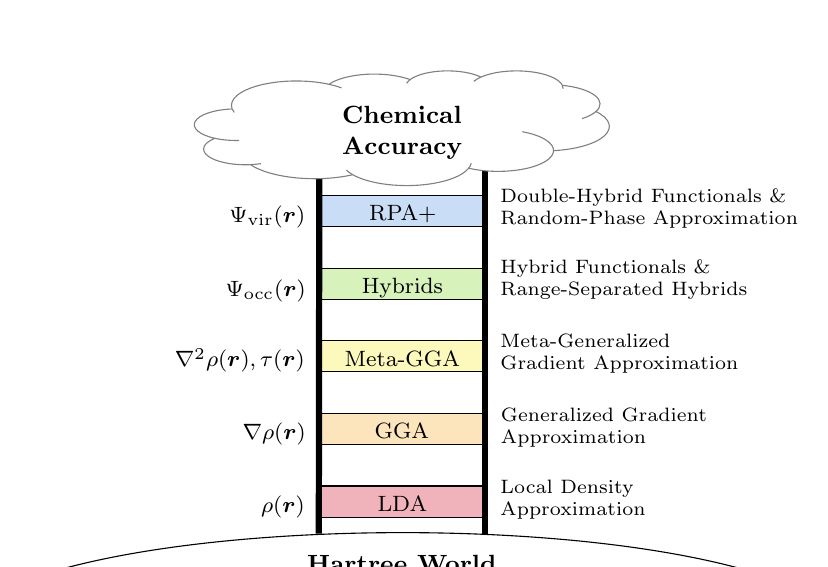
\begin{tikzpicture}[x=0.75pt,y=0.75pt,yscale=-1,xscale=1]
%Curve Lines [id:da86891233878799] 
\draw    (29,246) .. controls (114.03,216.08) and (303.78,215.83) .. (389,246) ;
%Shape: Rectangle [id:dp6440602598272736] 
\draw  [fill={rgb, 255:red, 241; green, 179; blue, 187 }  ,fill opacity=1.0 ] (169,201) -- (249,201) -- (249,216) -- (169,216) -- cycle ;
%Shape: Rectangle [id:dp16390793343447418] 
\draw  [fill={rgb, 255:red, 252; green, 228; blue, 189 }  ,fill opacity=1.0 ] (169,166) -- (249,166) -- (249,181) -- (169,181) -- cycle ;
%Shape: Rectangle [id:dp44785830951060834] 
\draw  [fill={rgb, 255:red, 253; green, 248; blue, 187 }  ,fill opacity=1.0 ] (169,131) -- (249,131) -- (249,146) -- (169,146) -- cycle ;
%Shape: Rectangle [id:dp38853804770808686] 
\draw  [fill={rgb, 255:red, 216; green, 242; blue, 188 }  ,fill opacity=1.0 ] (169,96) -- (249,96) -- (249,111) -- (169,111) -- cycle ;
%Shape: Rectangle [id:dp45002736761667594] 
\draw  [fill={rgb, 255:red, 201; green, 222; blue, 246 }  ,fill opacity=1.0 ] (169,61) -- (249,61) -- (249,76) -- (169,76) -- cycle ;
%Straight Lines [id:da9515996496239052] 
\draw [line width=2.25]    (169.26,32.59) -- (169,224) ;
%Straight Lines [id:da24533370255825981] 
\draw [line width=2.25]    (249,36) -- (249,224) ;
%Shape: Cloud [id:dp33766008859162566] 
\draw  [color={rgb, 255:red, 128; green, 128; blue, 128 }  ,draw opacity=1 ][fill={rgb, 255:red, 255; green, 255; blue, 255 }  ,fill opacity=1 ] (127.2,19.2) .. controls (125.59,14.74) and (130.88,10.33) .. (140.82,7.83) .. controls (150.76,5.34) and (163.61,5.2) .. (173.92,7.47) .. controls (177.57,4.88) and (184.26,3.09) .. (191.95,2.65) .. controls (199.65,2.2) and (207.45,3.15) .. (213,5.21) .. controls (216.1,2.86) and (222.21,1.28) .. (229.15,1.03) .. controls (236.09,0.79) and (242.88,1.91) .. (247.1,3.99) .. controls (252.72,1.5) and (261.66,0.45) .. (270.06,1.3) .. controls (278.45,2.15) and (284.79,4.74) .. (286.33,7.95) .. controls (293.22,8.66) and (298.96,10.46) .. (302.06,12.88) .. controls (305.16,15.3) and (305.33,18.12) .. (302.52,20.59) .. controls (309.3,23.91) and (310.88,28.34) .. (306.68,32.22) .. controls (302.48,36.1) and (293.13,38.85) .. (282.11,39.44) .. controls (282.03,43.08) and (276.73,46.43) .. (268.24,48.18) .. controls (259.75,49.93) and (249.41,49.82) .. (241.2,47.89) .. controls (237.7,52.26) and (227.85,55.47) .. (215.91,56.14) .. controls (203.97,56.81) and (192.08,54.82) .. (185.36,51.03) .. controls (177.14,52.9) and (167.27,53.43) .. (157.99,52.52) .. controls (148.7,51.61) and (140.78,49.32) .. (136.01,46.18) .. controls (127.6,46.55) and (119.48,44.91) .. (115.66,42.07) .. controls (111.85,39.24) and (113.16,35.81) .. (118.94,33.49) .. controls (111.44,31.83) and (107.62,28.53) .. (109.46,25.32) .. controls (111.3,22.11) and (118.39,19.71) .. (127.03,19.37) ; \draw  [color={rgb, 255:red, 128; green, 128; blue, 128 }  ,draw opacity=1 ] (118.94,33.49) .. controls (122.48,34.27) and (126.57,34.63) .. (130.65,34.51)(136.01,46.18) .. controls (137.76,46.1) and (139.49,45.94) .. (141.13,45.69)(185.36,51.03) .. controls (184.13,50.33) and (183.09,49.58) .. (182.28,48.8)(241.2,47.89) .. controls (241.84,47.1) and (242.25,46.28) .. (242.43,45.45)(282.11,39.44) .. controls (282.19,35.57) and (276.34,32.02) .. (267.07,30.32)(302.52,20.59) .. controls (301.01,21.91) and (298.72,23.08) .. (295.82,24.01)(286.33,7.95) .. controls (286.59,8.48) and (286.71,9.02) .. (286.69,9.57)(247.1,3.99) .. controls (245.7,4.61) and (244.55,5.31) .. (243.67,6.05)(213,5.21) .. controls (212.25,5.77) and (211.69,6.37) .. (211.33,6.99)(173.92,7.47) .. controls (176.1,7.95) and (178.12,8.53) .. (179.93,9.2)(127.2,19.2) .. controls (127.42,19.81) and (127.77,20.42) .. (128.25,21.01) ;
% Text Node
\draw (209.25,30.75) node  [font=\small] [align=left] {\textbf{Chemical}\\\textbf{Accuracy}};
% Text Node
\draw (255.25,196.75) node [anchor=north west][inner sep=0.75pt]  [font=\scriptsize] [align=left] {Local Density \\Approximation};
% Text Node
\draw (255.5,162) node [anchor=north west][inner sep=0.75pt]  [font=\scriptsize] [align=left] {Generalized Gradient \\Approximation};
% Text Node
\draw (255.25,126.5) node [anchor=north west][inner sep=0.75pt]  [font=\scriptsize] [align=left] {Meta-Generalized \\Gradient Approximation};
% Text Node
\draw (255.25,91) node [anchor=north west][inner sep=0.75pt]  [font=\scriptsize] [align=left] {Hybrid Functionals \&\\ Range-Separated Hybrids};
% Text Node
\draw (209.5,75.5) node [anchor=south] [inner sep=0.75pt]  [font=\footnotesize] [align=left] {RPA+};
% Text Node
\draw (209.25,214.5) node [anchor=south] [inner sep=0.75pt]  [font=\footnotesize] [align=left] {LDA};
% Text Node
\draw (209,179.25) node [anchor=south] [inner sep=0.75pt]  [font=\footnotesize] [align=left] {GGA};
% Text Node
\draw (209.25,144.55) node [anchor=south] [inner sep=0.75pt]  [font=\footnotesize] [align=left] {Meta-GGA};
% Text Node
\draw (209.25,111.4) node [anchor=south] [inner sep=0.75pt]  [font=\footnotesize] [align=left] {Hybrids};
% Text Node
\draw (255.25,56.5) node [anchor=north west][inner sep=0.75pt]  [font=\scriptsize] [align=left] {Double-Hybrid Functionals \&\\ Random-Phase Approximation};
% Text Node
\draw (163.5,217.6) node [anchor=south east] [inner sep=0.75pt]  [font=\footnotesize]  {$\rho (\bm{r})$};
% Text Node
\draw (164,182.6) node [anchor=south east] [inner sep=0.75pt]  [font=\footnotesize]  {$\nabla \rho (\bm{r})$};
% Text Node
\draw (163.5,147.6) node [anchor=south east] [inner sep=0.75pt]  [font=\footnotesize]  {$\nabla ^{2} \rho (\bm{r}) ,\tau (\bm{r})$};
% Text Node
\draw (164,113.6) node [anchor=south east] [inner sep=0.75pt]  [font=\footnotesize]  {$\Psi _{\text{occ}}(\bm{r})$};
% Text Node
\draw (163.75,77.85) node [anchor=south east] [inner sep=0.75pt]  [font=\footnotesize]  {$\Psi _{\text{vir}}(\bm{r})$};
% Text Node
\draw (209,244.15) node [anchor=south] [inner sep=0.75pt]  [font=\small] [align=left] {\textbf{Hartree World}};
\end{tikzpicture}
\onehalfspacing
\caption[Example Figure \#1: \texttt{tikz} example of Perdew's Ladder.]{Example Figure \#1: Here I include a \texttt{tikz} example of Perdew's Ladder \cite{perdew2001jacob}. The \texttt{tikz} package lets you use LaTeX code to generate beautiful vector graphics using standard LaTeX sizes and fonts. This also prevents graphics from being compressed and drastically reduces the file size of your thesis. I generated many graphics in my thesis using \href{https://www.mathcha.io}{( www.mathcha.io )}, and I cannot recommend it enough. \label{F2.1}}
\end{figure}


%~~~~~~~~~~~~~~~~~~~~~~~~~~~~~~~~~~~~~~~~~~~~~~~~~~~~~~~~~~~~~~~~~~~~~~~~~~~~~~~~~~~~~~~~~~~~~~~~
\chapter[The title of your publication that has been inserted as a chapter in the main body of your thesis]{Short Paper Title Suitable for Chapter Heading} 
\chaptermark{Short Paper Title Suitable for Chapter Heading}
\label{Oscallot} \thispagestyle{Chapter}
%~~~~~~~~~~~~~~~~~~~~~~~~~~~~~~~~~~~~~~~~~~~~~~~~~~~~~~~~~~~~~~~~~~~~~~~~~~~~~~~~~~~~~~~~~~~~~~~~
\begin{quote}
\textsl{``The career of a young theoretical physicist consists of treating the harmonic oscillator in ever-increasing levels of abstraction.''} \cite{coleman2019lectures} \\ 
$\sim$ Prof.\@ Sidney Coleman (1937--2007) 
\end{quote}
\vspace*{1cm}
{
\noindent \color{darkgray} 
This chapter is adapted from: \textbf{Bryenton, K.\@ R.\@}, \& Johnson, E.\@ R.\@ \textit{Many-Body Dispersion in Model Systems and the Sensitivity of Self-Consistent Screening}.\@ J.\@ Chem.\@ Phys.\@, \textbf{158}, 20, 204110.\@ (2023) \cite{bryenton2023many}\\
\smallskip\\
Author contributions: K.R.B.\ developed the mathematical model, wrote the software, generated all data, and wrote the first draft of the manuscript.
}
\clearpage
\section{Main Body Chapter Suggestions} \label{Ch3:Suggestions}

Here we show an example of including a published paper into your thesis. I suggest making a ``cover page'' with the title of the article and a list of author contributions. Then you can copy-and-paste the \texttt{.tex} file (using your latest preprint, rather than the gallery proof) into your thesis. I also suggest not including the introductions from each paper, as this should already be covered in your theory chapters. Instead, include new information only and edit the initial sections of the paper to flow nicely with the previous chapters of the thesis.


In many cases, your article titles will be too long to elegantly display. Here, we effectively use three titles for this chapter: \texttt{\textbackslash chapter[TOC Display]\{Chapter Display\} \textbackslash chaptermark\{Header Display\}}. The ``TOC Display'' is used to control what this chapter is called in your Table of Contents, and I suggest using the full title of your article. ``Chapter Display'' is used after the ``Chapter 3'' heading on the previous page, and ``Header Display'' is used in the header of the same page. I prefer to set ``Chapter Display'' and ``Header Display'' to the same thing, and use shorter versions of the full article title.  




%~~~~~~~~~~~~~~~~~~~~~~~~~~~~~~~~~~~~~~~~~~~~~~~~~~~~~~~~~~~~~~~~~~~~~~~~~~~~~~~~~~~~~~~~~~~~~~~~
\chapter[Conclusions]{Conclusions} \label{Conclusions} \thispagestyle{Chapter}
%~~~~~~~~~~~~~~~~~~~~~~~~~~~~~~~~~~~~~~~~~~~~~~~~~~~~~~~~~~~~~~~~~~~~~~~~~~~~~~~~~~~~~~~~~~~~~~~~
\begin{quote}
\textsl{``One never notices what has been done; one can only see what remains to be done.''} \cite{ratcliffe2014oxford} \\ 
$\sim$ Prof.\@ Marie Curie (1867--1934) 
\end{quote}
\vspace*{1cm}



\section{Dissertation Summary} \label{Ch4:Summary}

For the summary, you can walk through each chapter, briefly summarizing the findings and connecting them to convey a common theme.


\section{Future Work} \label{Ch4:FutureWork}

For future work, consider trying to find 2--3 new avenues your research could progress. Each one can become its own subsection.

\clearpage











%~~~~~~~~~~~~~~~~~~~~~~~~~~~~~~~~~~~~~~~~~~~~~~~~~~~~~~~~~~~~~~~~~~~~~~~~~~~~~~~~~~~~~~~~~~~~~~~~
\clearpage
\interlinepenalty=10000	    % Forces no pagebreaks in bibliography entries
\pagestyle{Chapter} 	    % Without, this will make last page of bibliography have \pagestyle{body}
\singlespacing              % FGS requests single spacing in bib, 1.5 or 2.0 between entries
{\sloppy \printbibliography[heading=bibintoc, title={Bibliography}] }%This adds Bibliography to ToC
\onehalfspacing             % Switch back to default
\interlinepenalty=0    	    % Switch back to default
\pagestyle{Body}   		    % Switch back to default
\clearpage 
%~~~~~~~~~~~~~~~~~~~~~~~~~~~~~~~~~~~~~~~~~~~~~~~~~~~~~~~~~~~~~~~~~~~~~~~~~~~~~~~~~~~~~~~~~~~~~~~~




%~~~~~~~~~~~~~~~~~~~~~~~~~~~~~~~~~~~~~~~~~~~~~~~~~~~~~~~~~~~~~~~~~~~~~~~~~~~~~~~~~~~~~~~~~~~~~~~~
\appendix 
\chapter{Chapter 1 Supplement} \label{A:C1sup} \thispagestyle{Chapter}
%~~~~~~~~~~~~~~~~~~~~~~~~~~~~~~~~~~~~~~~~~~~~~~~~~~~~~~~~~~~~~~~~~~~~~~~~~~~~~~~~~~~~~~~~~~~~~~~~

Content that distracts from the flow of the dissertation, or relevant material included in the ESI of your articles, is normally placed in the appendices. Here, I've broken the appendix into ``supplements'' for each chapter, but this is just a personal preference.


\begin{figure}[h!] % PERDEW'S LADDER
\centering
\includegraphics[width=0.6\textwidth]{example-image}
\caption[Example Figure \#2: An example using \texttt{includegraphics}.]{Example Figure \#2: Here is a figure example where we import the graphic using \texttt{includegraphics} rather than \texttt{input}.  \label{FA.1}}
\end{figure}



\chapter{Chapter 2 Supplement} \label{A:C2sup} \thispagestyle{Chapter}


\section{Common Unit Conversion Factors} \label{A:Units}

\begin{table}[h]
\centering
\caption[Example Table: Conversion factors between common units used in electronic structure theory.]{Example Table: Conversion factors between common energy units used in electronic structure theory to six significant figures. Units include: Hartree (Ha.), electronvolt (eV), kilocalorie per mole (kcal/mol), kilojoule per mole \mbox{(kJ/mol)}, and wavenumber (cm$^{-1}$). To convert from a row unit to a column unit, multiply by the corresponding table entry. For commonly used units of length, note that $1~\text{\AA} = 10^{-10}~\text{m} \approx 1.88973~\text{bohr}$. Values were obtained from Ref.~\cite{rumble2021crc}.}
\begin{tabular}{r | lllll}
\hline
           & Ha.                     & eV                      & kcal/mol                & kJ/mol                  & cm$^{-1}$ \\ \hline
 Ha.       & 1                       & 27.2114                 & 627.510                 & 2625.50                 &  219475   \\
 eV        & 3.67493$\times 10^{-2}$ & 1                       & 23.0605                 & 96.4853                 & 8065.54   \\             
 kcal/mol  & 1.59360$\times 10^{-3}$ & 4.33641$\times 10^{-3}$ & 1                       & 4.18400                 & 349.755   \\             
 kJ/mol    & 3.80880$\times 10^{-4}$ & 1.03643$\times 10^{-3}$ & 2.39006$\times 10^{-1}$ & 1                       & 83.5935   \\             
 cm$^{-1}$ & 4.55634$\times 10^{-6}$ & 1.23984$\times 10^{-4}$ & 2.85914$\times 10^{-3}$ & 1.19627$\times 10^{-3}$ & 1         \\ \hline
 \end{tabular}
\end{table}


\end{document}
